\documentclass[12pt,letterpaper]{article}
\usepackage{amsmath,amsthm,amsfonts,amssymb,amscd}
\usepackage{fullpage}
\usepackage{graphicx}
\usepackage{lastpage}
\usepackage{listings}
\lstset{
	numbers=left,
	numbersep=5pt,
	stepnumber=1,
	tabsize=2,
	showstringspaces=false
}
\usepackage{enumerate}
\usepackage{fancyhdr}
\usepackage{hyperref}
\usepackage{mathrsfs}
\usepackage{cancel}
\usepackage{xcolor}
\usepackage[margin=3cm]{geometry}
\setlength{\parindent}{0.0in}
\setlength{\parskip}{0.05in}

% Edit these as appropriate
\newcommand\course{STA561/CS571}
\newcommand\semester{Fall 2013}     % <-- current semester
\newcommand\hwnum{5}                  % <-- homework number
\newcommand\yourname{Matt Dickenson} % <-- your name
\newcommand\login{mcd31}           % <-- your NetID
\newcommand\hwdate{Due: 28 October, 2013}           % <-- HW due date

\newenvironment{answer}[1]{
  \subsubsection*{Problem #1}
}


\pagestyle{fancyplain}
\headheight 35pt
\lhead{\yourname\ \texttt{\login}\\\course\ --- \semester}
\chead{\textbf{\Large Homework \hwnum}}
\rhead{\hwdate}
\headsep 10pt

\begin{document}

\noindent \emph{Homework Notes:} I did not work with anyone else on this homework or refer to resources other than the course notes, textbook, and course Piazza page.

\begin{answer}{1}

\paragraph{A} Figure \ref{eigens} shows the distribution of eigenvalues for each matrix covariance matrix of $X$ with different values of $\psi$ ($X_i$ uses $\psi_i$). All of the distributions are right-skewed, but the mean of the eigenvalues increases and the variance decreases as the amount of noise ($\psi$) in the original matrix increases. The eigenvalues were normalized using the $\ell^2$ norm. 

\begin{figure}[h!]
\begin{center}
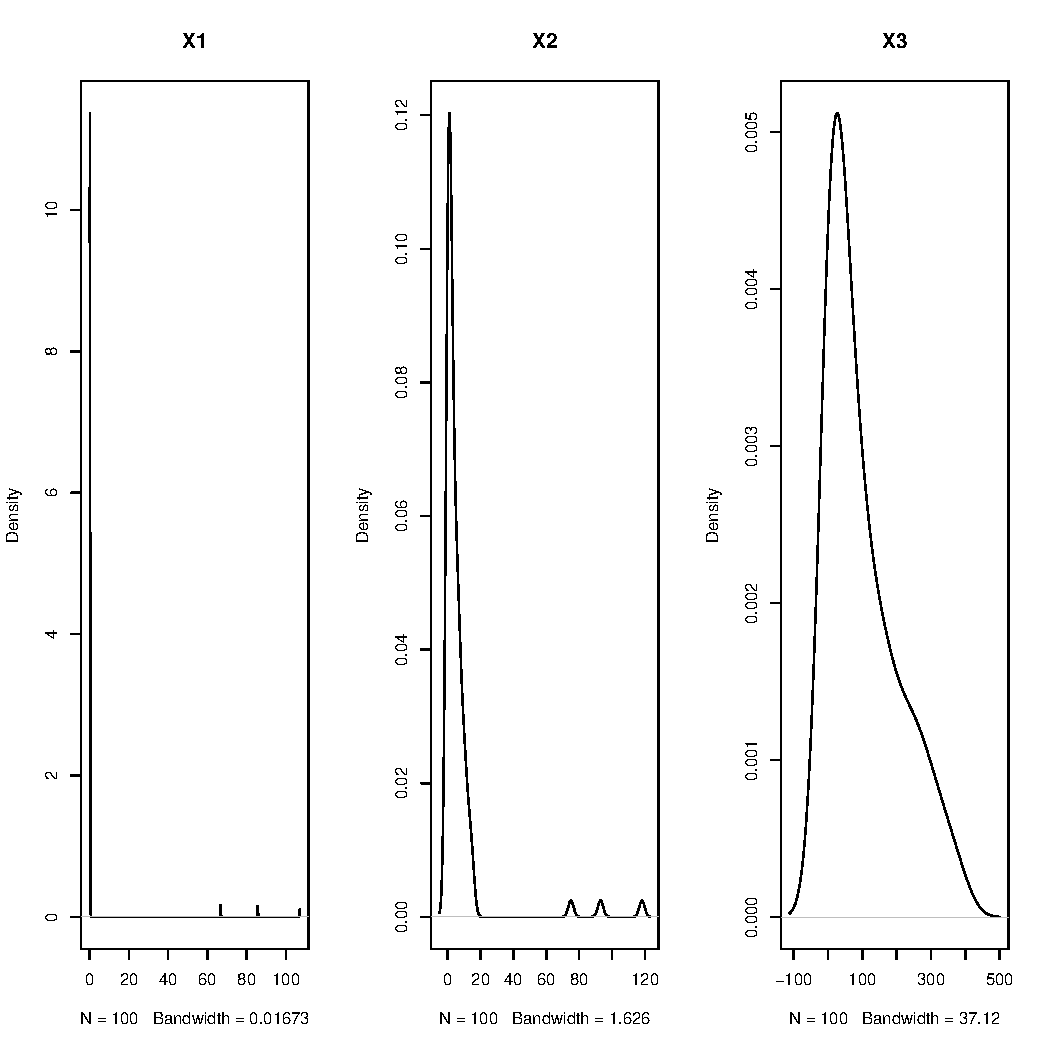
\includegraphics[scale=0.5]{1a.pdf}
\caption{Distribution of Normalized Eigenvalues for Three Values of $\psi$}
\label{eigens}
\end{center}
\end{figure}

\paragraph{B} Table \ref{rmse} presents the root mean squared error (RMSE) between the covariances of the X matrices and the matrix reconstructions using the first three eigenvectors (and eigen values). Overall, the eigenvectors do a good job of recapitulating the original data matrices. Those with less noise (small $\psi$) do a better job (lower RMSE) than those with more noise. 

\begin{table}[h!]
\begin{center}
\caption{RMSE between Cov(X) and Matrix Reconstructions}
\label{rmse}
\begin{tabular}{cr}
$\psi$ & \texttt{RMSE} \\
\hline
0.2 & 0.0054 \\
2 & 0.553 \\
10 & 13.029
\end{tabular}
\end{center}
\end{table}

\paragraph{C} When we reconstruct the matrices we are able to obtain an estimate of the covariance of $X$, subject to some noise. This could be useful for identifying the number of components that could be used in our analysis, as long as we assume that the level of noise is relatively low. 

\end{answer}

\begin{answer}{2}

\paragraph{A and B}


Steps for building string kernel:
\begin{enumerate}
\item Create all possible ``words'' up to length three (3) using the letters A, C, G, and T (\texttt{combos})
\item Write a function to count all occurrences of a substring within a string (\texttt{substringCount})
\item Write a string kernel function to loop through the words generated in step 1, count their occurrence within a string using the function in step 2, multiply, and apply a weight proportional to the length of the word/substring (\texttt{stringKernel}) 
\end{enumerate}

The $(i,j)^{th}$ Gram matrix entry, $K(x_i, x_j)$ was computed as $\Sigma_a w(a) \phi(x_i, a) \phi(x_2, a)$ where $a$ is a word/substring, $\phi(x, a)$ counts the occurrences of $a$ in $x$, and $w(a) = {|a| \over 228}$ because there are a total of 228 characters in all the words that can be created as a combination of A, C, G, and T. 

\lstinputlisting[language=R, caption=R Code for 2A and 2B, firstline=76, lastline=149, firstnumber=1]{cs571-hw5.r}


\paragraph{C}

Figure \ref{scatter} presents a scatter plot of predicted intensities versus the measured intensities in the test data. The RMSE was calculated to be 0.654. 

\begin{figure}
\begin{center}
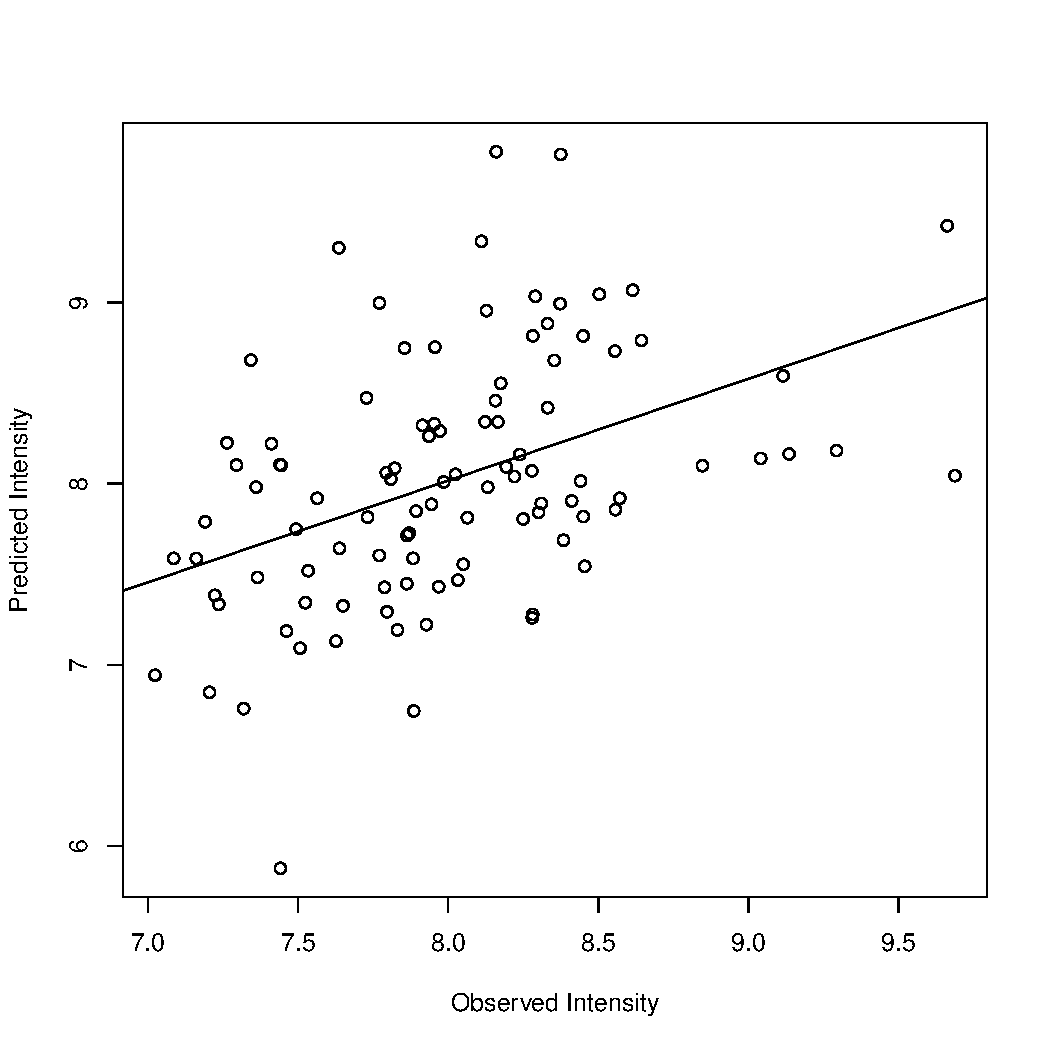
\includegraphics{scatterplot.pdf}
\caption{Scatterplot of Predicted versus Measured Intensities}
\label{scatter}
\end{center}
\end{figure}

\paragraph{D} There are at least three ways that we would improve the prediction acuracy for our regression:

\begin{enumerate}
\item Consider longer substrings of the sequence, such as $|A|={4,5,...}$
\item Modify the weights put on shorter substrings, including weighting single character strings at zero
\item Try other values of $\sigma$
\end{enumerate}

\end{answer}


\end{document}